\documentclass{report}

% Input packages & formatting
% Packages

% Math packages
\usepackage{amsmath} % Extended math functions
\usepackage{amssymb} % Extended math symbols (loads in amsfonts)
\usepackage{bm} % Bold math symbols
\usepackage{mathtools}

% Figure packages
\usepackage{caption} % Caption formatting for university standard
\usepackage{graphicx} % includegraphics command
\usepackage{subcaption} % Subfigures
\usepackage[section]{placeins} % Place floats in section
\usepackage{wrapfig}

% Table packages
\usepackage{booktabs} % Better tables
\usepackage{bigstrut} % Merged table cells
\usepackage{longtable} % Tables which overflow into next page
\usepackage{array}
\usepackage{colortbl} % Color table cells
\usepackage{makecell}
\usepackage{multirow}

% Fonts
\usepackage{lmodern} % Use latin modern rather than computer modern. Better for font encoding.
\usepackage[T1]{fontenc} % Allow text to be searchable in output

% Other packages
\usepackage{appendix} % Appendix environment
\usepackage{nextpage} % Cleartooddpage command
%\usepackage[square,comma,sort,numbers]{natbib} % Reference formatting
\usepackage{setspace} % Line spacing
\usepackage{listings} % Display code with syntax highlighting
\usepackage{upquote} % Vertical quotes in verbatim
\usepackage{xcolor} % Colors
\usepackage{titlesec} % Header spacing
\usepackage{xparse} % for tcolorbox
\usepackage[listings]{tcolorbox} % Colored boxes for highlighting syntax
\tcbuselibrary{breakable}
\tcbuselibrary{skins}
\usepackage{enumitem} % better enumerate/itemize options
\usepackage{fancyhdr}
\usepackage{multicol}
\usepackage{ifthen}
\usepackage{xstring}

% Table of contents
\usepackage{imakeidx} % Index page
\usepackage{tocloft} % Control of table of contents
\usepackage[nottoc]{tocbibind} % Adds bibliography, table of tables, table of figures, to table of contents
\usepackage[bookmarks,linktocpage,hidelinks]{hyperref} % Hyperlinks for sections, figures, etc.
\usepackage{nameref}

% Bibliography
\usepackage[style=numeric,backend=bibtex]{biblatex}
\addbibresource{references/references.bib}

% Formatting
% Page format
\setlength{\oddsidemargin}{0.00in}  % Left side margin for odd numbered pages
\setlength{\evensidemargin}{0.00in} % Right side margin for even numbered pages
\setlength{\topmargin}{0.00in}      % Top margin
\setlength{\headheight}{0.20in}     % Header height
\setlength{\headsep}{0.20in}        % Separation between header and main text
\setlength{\topskip}{0.00in}        % Top skip
\setlength{\textwidth}{6.50in}      % Width of the text
\setlength{\textheight}{8.50in}     % Height of the text
\setlength{\footskip}{0.50in}       % Foot skip
\setlength{\parindent}{0.00in}      % First line indentation
\setlength{\parskip}{6pt}        % Space between two paragraphs

% Captions (figures, tables, etc.)
\setlength{\floatsep}{\parskip}          % Space left between floats.
\setlength{\textfloatsep}{\floatsep}   % Space between last top float
% or first bottom float and the text
\setlength{\intextsep}{\floatsep}      % Space left on top and bottom
% of an in-text float
\setlength{\abovecaptionskip}{0.1in plus 0.25in}  % Space above caption
\setlength{\belowcaptionskip}{0.1in plus 0.25in}  % Space below caption
\setlength{\captionmargin}{0.50in}     % Left/Right margin for caption
\setlength{\abovedisplayskip}{0.00in plus 0.25in} % Space before Math stuff
\setlength{\belowdisplayskip}{0.00in plus 0.25in} % Space after Math stuff
\setlength{\arraycolsep}{0.10in}       % Gap between columns of an array
\setlength{\jot}{0.10in}                % Gap between multiline equations
\setlength{\itemsep}{0.10in}           % Space between successive items

% Counters (no section numbering)
\setcounter{tocdepth}{3}
\setcounter{secnumdepth}{0}

% Spacing
\setstretch{1.5}

\titlespacing*{\chapter}{0cm}{6pt}{6pt}[0cm]
\titlespacing*{\section}{0cm}{6pt}{6pt}[0cm]
\titlespacing*{\subsection}{0cm}{6pt}{6pt}[0cm]
\titlespacing*{\subsubsection}{0cm}{6pt}{6pt}[0cm]

\renewcommand{\contentsname}{\sffamily\bfseries\Huge{Contents}}
\titleformat{\chapter}
{\sffamily\bfseries\Huge}{}{0pt}{\thechapter. }
\titleformat{name=\chapter,numberless}
{\sffamily\bfseries\Huge}{}{0pt}{}
\titleformat{\section}
{\sffamily\huge}{}{0pt}{\titlerule\vspace{-0.2cm}}
\titleformat{\subsection}
{\sffamily\itshape\Large}{}{0pt}{}

% Macro for syntax
\newtcolorbox{syntax}{
    size=small,
    sharp corners,
    colframe=black,
    colback=yellow,
    fontupper=\bfseries\ttfamily
}

% Macro for argument table
\newenvironment{args}{
    \begin{tabular}{>{\bfseries\ttfamily}p{0.25\linewidth} p{0.69\linewidth}}
    }{
    \end{tabular}\par
    \vspace{0.5\baselineskip}
}

% Note: Requires packages "listing", "xcolor", and "textcomp"
\lstdefinelanguage{verbatim}{
    basicstyle=\ttfamily\small,
    xleftmargin=9pt,
    xrightmargin=9pt,
    columns=fullflexible,
    keepspaces=true,
    breaklines=true
}

% Example code
\AtBeginDocument{
\newtcolorbox[blend into=listings]{example}[2][]{
    colback=blue!3!white,
    colframe=black,
    colbacktitle=blue!15!white,
    coltitle=black,
    sharp corners,
    enhanced,
    breakable,
    size=small,
    before upper={
        \setstretch{1.0}\lstset{language=verbatim}\vspace{3pt}\textsf{\textit{Code:}}
    },
    subtitle style={
        colback=blue!20!white,
        fonttitle=\sffamily
    },
    before lower={
        \setstretch{1.0}\lstset{language=verbatim}\vspace{3pt}\textsf{\textit{Output:}}
    },
    fonttitle=\sffamily,
    title={#2},
    #1
}
}
\newcommand{\moduleinfo}[1]{ %
\rule{\linewidth}{1pt}\\
\begin{tabular}{c l l}
\multirow{2}{0.1in}{
\includegraphics[height=0.5in]{arrow_vert}} & Package: & tda::#1 \\
& Version: & \version[#1]
\end{tabular}\\
\rule{\linewidth}{1pt}
}

% Links to sub and subsub commands - optional boolean argument, default true. if false, only displays subcmd.

% Commands (and command ensembles)
\newcommand{\command}[1]{\protect\hypertarget{#1}{#1}\index{#1}}
\newcommand{\subcommand}[2]{\protect\hypertarget{#1 #2}{#1 #2}\index{#1!#2}}
\newcommand{\cmdlink}[1]{\protect\hyperlink{#1}{\textit{#1}}}
\newcommand{\subcmdlink}[3][1]{\protect\hyperlink{#2 #3}{\ifnum#1=1\relax\textit{#2 #3}\else\textit{#3}\fi}}

% Methods (first arg is class)
\newcommand{\method}[2]{\protect\hypertarget{$#1Obj #2}{\$#1Obj #2}\index{#1 methods!#2}}
\newcommand{\methodlink}[3][1]{\protect\hyperlink{$#2Obj #3}{\ifnum#1=1\relax\textit{\$#2Obj #3}\else\textit{#3}\fi}}

% Macros for figure/table names
\newcommand{\fig}{\figurename\ }
\newcommand{\figs}{\figurename s }
\newcommand{\tbl}{\tablename\ }
\newcommand{\tbls}{\tablename s }
\newcommand{\eq}{Eq. }
\newcommand{\eqs}{Eqs. }
\renewcommand{\lstlistingname}{Example}% Listing -> Example
\renewcommand{\lstlistlistingname}{List of \lstlistingname s}% List of Listings -> List of Examples
\newcommand{\ex}{Example }
\newcommand{\exs}{Examples }
\newcommand{\var}[1]{\texttt{\textbf{\$#1}}}

% Changes to referencing
\numberwithin{equation}{chapter}
\renewcommand{\theequation}{\thechapter-\arabic{equation}}
\AtBeginDocument{
    \numberwithin{lstlisting}{chapter}
    \renewcommand{\thelstlisting}{\thechapter.\arabic{lstlisting}}
}

% Header/footer
\renewcommand{\headrulewidth}{0pt}

\fancypagestyle{main}{
\fancyhf{}
\fancyhead[RE,LO]{\textsf{\nouppercase \leftmark}}
\fancyhead[LE,RO]{\textsf{\thepage}}
}

\fancypagestyle{chapter}{
\fancyhf{}
\fancyfoot[LE,RO]{\textsf{\thepage}}
}

\fancypagestyle{foreword}{
\fancyhf{}
\fancyfoot[C]{\textsf{\thepage}}
}

% Changes to hyperlinks (URLs)
\renewcommand\UrlFont{\color{blue}\rmfamily}

% New column type 
% https://tex.stackexchange.com/questions/75717/how-can-i-mix-itemize-and-tabular-environments
\newcolumntype{L}{>{\labelitemi~~}l<{}}
\newcommand{\version}[1][]{\IfStrEqCase{#1}{%
{}{0.1.2}%
{ndlist}{0.1.0}%
{tbl}{0.1.0}%
{io}{0.1.0}%
{vis}{0.1.1}%
}}

\renewcommand{\cleartooddpage}[1][]{\ignorespaces} % single side
\newcommand{\caret}{$^\wedge$}

% Other macros
\renewcommand{\^}[1]{\textsuperscript{#1}}
\renewcommand{\_}[1]{\textsubscript{#1}}

% Figure path and type
\pdfminorversion=6
\DeclareGraphicsExtensions{.pdf,.png}
\graphicspath{{./figures/}}

\title{\Huge{Tcl Data Analysis (Tda)}\\\large Version \version}
\author{Alex Baker\\\small\hyperlink{https://github.com/ambaker1/tda}{https://github.com/ambaker1/tda}}
\date{\small\today}
\makeindex[columns=3,title={Command Index}]

\begin{document}
    \maketitle
    \begin{abstract}
    Tda (pronounced "tada") provides data analysis tools for use in Tcl scripts. It adds native n-dimensional arrays, a tabular datatype, file import/export and datatype conversion utilities, and data visualization tools to Tcl. Tda was originally developed for OpenSees users, but can be used in any Tcl application.
    \end{abstract}
    \fancypagestyle{plain}[foreword]{}
    \pagestyle{plain}
    \cleartooddpage[\thispagestyle{empty}]
    \pagenumbering{roman}
    \tableofcontents
    \markboth{}{}
    \cleartooddpage[\thispagestyle{empty}]
    \fancypagestyle{plain}[chapter]{}
    \pagestyle{main}
    \pagenumbering{arabic}
    \chapter*{Introduction to Tda}
\addcontentsline{toc}{chapter}{Introduction to Tda}  
Tda (pronounced "ta-da!"), which stands for ``Tcl Data Analysis'', adds features such as N-dimensional arrays and tabular data structures to Tcl. 
Tda was originally developed for OpenSees, an open-source scripting-based finite-element analysis software, specializing in earthquake engineering simulation \cite{mazzoni_opensees_2006,mckenna_nonlinear_2010}, but it is general enough for any Tcl application. 

Tda version \version\ contains the following sub-packages and their respective versions:

\begin{tabular}{lll}
Package & Version & Description \\
\hline
 tda::ndlist & \version[ndlist] & \nameref{ndlist}\\
 tda::tbl & \version[tbl] & \nameref{tbl}\\
 tda::io & \version[io] & \nameref{io}\\
 tda::vis & \version[vis] & \nameref{vis}
\end{tabular}

\clearpage
\section{Notation}
This manual is for Tcl commands, and the notation style is as follows:
\begin{itemize}
\item The prefix \texttt{\$} is used to denote an input variable, and all other words are literal strings.
\item Option keywords are typically denoted with the prefix \texttt{-}, and all optional inputs are denoted by enclosing in \texttt{<>} braces.
\item An arbitrary number of arguments is denoted by ``1 2 ...'' notation, (e.g. \texttt{\$arg1 \$arg2 ...}), unless if the arguments must be paired, in which case it will use a ``key value ...'' notation.
\end{itemize}
Below is an example of the notation used for commands in this manual.
\begin{syntax}
command \$foo <-bar> <\$key \$value ...>
\end{syntax}
\begin{args}
\$foo & Required variable input ``foo''. \\
-bar & Optional keyword ``-bar''. \\
\$key \$value ... & Optional paired list (arbitrary number of pairs).
\end{args}

\clearpage
\section{Loading and Importing Tda Commands}
Tda is organized into modules, each contained within a unique namespace and package name, prefixed with \textit{tda}, the parent namespace/package. 
Loading the main \textit{tda} package using  \textit{package require} loads all the modules.
Alternatively, modules can be individually loaded by specifying the module package names.
\begin{syntax}
package require tda <\$version> \\
package require <-exact> tda::\$module <\$version>
\end{syntax}
\begin{args}
-exact & Option to require an exact version (must also include \$version). \\
\$module & Specific Tda module to require. \\
\$version & Specify minimum version number. Default highest stable version.
\end{args}
When Tda modules are loaded with \textit{package require}, procedures are created within the modules' respective namespaces. 
These commands can then be accessed with their fully-qualified names (such as \textit{tda::range}), or the commands can be imported with \textit{namespace import}, as shown below.
\begin{example}{Loading and importing Tda}
\begin{lstlisting}
package require tda
puts [tda::range 5]
namespace import tda::*
puts [range 5]
\end{lstlisting}
\tcblower
\begin{lstlisting}
0 1 2 3 4
0 1 2 3 4
\end{lstlisting}
\end{example}

\clearpage
\section{Object Oriented Tcl}
Some features in Tda (such as \textit{tda::tbl} tables) follow an object-oriented paradigm, using the built-in ``TclOO'' package. 
Additionally, all Tda widgets are object oriented, using the framework provided by the required package ``wob'' (\hyperlink{https://github.com/ambaker1/wob}{https://github.com/ambaker1/wob}).

In TclOO, a ``class'' command acts as a template for creating ``objects'', or commands that are linked to unique namespaces and have subcommands, or ``methods'' that allow for access and modification of variables in the object's namespace.
Since the TclOO package is utilized, all Tda classes have standard methods ``new'' and ``create'', and all Tda objects have the standard method ``destroy''.
Additionally, as TclOO is standard to Tcl 8.6 and above, class and object introspection using the \textit{info} command can be used to dive into the structure of the class (using its fully declared name) and its objects.

To demonstrate TclOO basics, see the example below of a fictitious class named ``foo''.
\begin{example}{TclOO basics}
\begin{lstlisting}
# Create objects from a class named 'foo'
set bar1 [foo new]; # Creates object with auto-generated name, storing in variable 'bar1'
foo create bar2; # Creates object with explicit command name 'bar2'
puts [info class instances foo]; # Display all instances of 'foo'
$bar1 destroy; # Destroys object stored in variable 'bar1'
bar2 destroy; # Destroys object 'bar2'
\end{lstlisting}
\tcblower
\begin{lstlisting}
::oo::Obj12 ::bar2
\end{lstlisting}
\end{example}
For a deeper dive into TclOO, check out the Tcl wiki page on it: \hyperlink{https://wiki.tcl-lang.org/page/TclOO}{https://wiki.tcl-lang.org/page/TclOO}

\cleartooddpage[\thispagestyle{empty}]
\section{Copyright and Disclaimer}
BSD 3-Clause License

Copyright (c) 2023, Alex Baker

Redistribution and use in source and binary forms, with or without
modification, are permitted provided that the following conditions are met:

1. Redistributions of source code must retain the above copyright notice, this
   list of conditions and the following disclaimer.

2. Redistributions in binary form must reproduce the above copyright notice,
   this list of conditions and the following disclaimer in the documentation
   and/or other materials provided with the distribution.

3. Neither the name of the copyright holder nor the names of its
   contributors may be used to endorse or promote products derived from
   this software without specific prior written permission.

THIS SOFTWARE IS PROVIDED BY THE COPYRIGHT HOLDERS AND CONTRIBUTORS "AS IS"
AND ANY EXPRESS OR IMPLIED WARRANTIES, INCLUDING, BUT NOT LIMITED TO, THE
IMPLIED WARRANTIES OF MERCHANTABILITY AND FITNESS FOR A PARTICULAR PURPOSE ARE
DISCLAIMED. IN NO EVENT SHALL THE COPYRIGHT HOLDER OR CONTRIBUTORS BE LIABLE
FOR ANY DIRECT, INDIRECT, INCIDENTAL, SPECIAL, EXEMPLARY, OR CONSEQUENTIAL
DAMAGES (INCLUDING, BUT NOT LIMITED TO, PROCUREMENT OF SUBSTITUTE GOODS OR
SERVICES; LOSS OF USE, DATA, OR PROFITS; OR BUSINESS INTERRUPTION) HOWEVER
CAUSED AND ON ANY THEORY OF LIABILITY, WHETHER IN CONTRACT, STRICT LIABILITY,
OR TORT (INCLUDING NEGLIGENCE OR OTHERWISE) ARISING IN ANY WAY OUT OF THE USE
OF THIS SOFTWARE, EVEN IF ADVISED OF THE POSSIBILITY OF SUCH DAMAGE.

    % Modules - alphabetic order
    \cleartooddpage[\thispagestyle{empty}]
\chapter{N-Dimensional List (ndlist) Module}
\moduleinfo{ndlist}
The ``ndlist'' module provides tools for list, matrix, and tensor manipulation and processing, where vectors are represented by Tcl lists, and matrices are represented by nested Tcl lists, and higher dimension lists represented by additional levels of nesting.

This datatype definition is consistent with the definition in the Tcllib math::linearalgebra package, which is the standard Tcl linear algebra library \cite{markus_tcl_2008}.

\clearpage

\section{Vectors (1D)}
Tcl provides numerous list manipulation utilities, such as \textit{lindex}, \textit{lset}, \textit{lrepeat}, and more.
Since vectors are simply Tcl lists, vectors can be created, accessed, and manipulated with standard Tcl list commands such as \textit{list}, \textit{lindex}, and \textit{lset}. 

The ndlist module provides additional vector creation and processing commands, especially for numerical lists.

\subsection{Range Generator}
The command \cmdlink{range} simply generates a range of integer values. There are two ways of calling this command, as shown below.
\begin{syntax}
\command{range} \$n \\
range \$start \$stop <\$step>
\end{syntax}
\begin{args}
\$n & Number of indices, starting at 0 (e.g. 3 returns 0 1 2). \\
\$start & Starting value. \\
\$stop & Stop value. \\
\$step & Step size. Default 1 or -1, depending on direction of start to stop.
\end{args}
\begin{example}{Integer range generation}
\begin{lstlisting}
puts [range 3]
puts [range 0 2]
puts [range 10 3 -2]
\end{lstlisting}
\tcblower
\begin{lstlisting}
0 1 2
0 1 2
10 8 6 4
\end{lstlisting}
\end{example}

\clearpage
\subsection{Generate Linearly Spaced Vector}
The command \cmdlink{linspace} can be used to generate a vector of specified length and equal spacing between two specified values. 
\begin{syntax}
\command{linspace} \$x1 \$x2 \$n
\end{syntax}
\begin{args}
\$x1 & Starting value \\
\$x2 & End value \\
\$n & Number of points
\end{args}
\begin{example}{Linearly spaced vector generation}
\begin{lstlisting}
puts [linspace 0 1 5]
\end{lstlisting}
\tcblower
\begin{lstlisting}
0.0 0.25 0.5 0.75 1.0
\end{lstlisting}
\end{example}
\subsection{Generate Fixed-Spacing Vector}
The command \cmdlink{linsteps} generates intermediate values given an increment size and a sequence of targets.
\begin{syntax}
\command{linsteps} \$step \$x1 \$x2 ...
\end{syntax}
\begin{args}
\$step & Maximum step size \\
\$x1 \$x2 ... & Targets to hit.
\end{args}
\begin{example}{Intermediate value vector generation}
\begin{lstlisting}
puts [linsteps 0.25 0 1 0]
\end{lstlisting}
\tcblower
\begin{lstlisting}
0 0.25 0.5 0.75 1 0.75 0.5 0.25 0
\end{lstlisting}
\end{example}
\clearpage
\subsection{Linear Interpolation}
The command \cmdlink{linterp} performs linear 1D interpolation.
\begin{syntax}
\command{linterp} \$xq \$xp \$yp
\end{syntax}
\begin{args}
\$xq & Vector of x values to query  \\
\$xp & Vector of x points, strictly increasing \\
\$yp & Vector of y points, same length as \texttt{\$xp}
\end{args}
\begin{example}{Linear interpolation}
\begin{lstlisting}
# Exact interpolation
puts [linterp 2 {1 2 3} {4 5 6}]
# Intermediate interpolation
puts [linterp 8.2 {0 10 20} {2 -4 5}]
\end{lstlisting}
\tcblower
\begin{lstlisting}
5
-2.92
\end{lstlisting}
\end{example}
\clearpage
\subsection{Logical Indexing}
The command \cmdlink{find} returns the indices of non-zero elements of a boolean vector, or indices of elements that satisfy a given criterion.
Can be used in conjunction with \cmdlink{nget} and its aliases to perform logical indexing.
\begin{syntax}
\command{find} <\$type> \$vector <\$op \$scalar>
\end{syntax}
\begin{args}
\$type & Search type. Default -all (returns list of matching indices). Other options are -first and -last, which return the first and last matching indices, or -1 if none are found. \\
\$vector & Boolean vector or vector of values to compare. \\
\$op & Comparison operator. Effectively default ``!=''. \\
\$scalar & Comparison value. Effectively default 0.
\end{args}

\begin{example}{Logical Indexing}
\begin{lstlisting}
puts [find {0 1 0 1 1 0}]
puts [find -first {0.5 2.3 4.0 2.5 1.6 2.0 1.4 5.6} > 2]
puts [find -last {0.5 2.3 4.0 2.5 1.6 2.0 1.4 5.6} > 2]
\end{lstlisting}
\tcblower
\begin{lstlisting}
1 3 4
1
7
\end{lstlisting}
\end{example}
\clearpage
\subsection{Dot Product}
The dot product of two vectors can be computed with \cmdlink{dot}. This function is based on the math::linearalgebra command \textit{dotproduct}.
\begin{syntax}
\command{dot} \$a \$b
\end{syntax}
\begin{args}
\$a & First vector. \\
\$b & Second vector. Must be same length as \texttt{\$a}.
\end{args}
\subsection{Cross Product}
The cross product of two vectors of length 3 can be computed with \cmdlink{cross}. This function is based on the math::linearalgebra command \textit{crossproduct}.
\begin{syntax}
\command{cross} \$a \$b
\end{syntax}
\begin{args}
\$a & First vector. Must be length 3.\\
\$b & Second vector. Must be length 3.
\end{args}

\subsection{Norm and Normalize}
The norm of a vector can be computed with \cmdlink{norm}, and a vector can be normalized (norm of 1) with \cmdlink{normalize}. These functions are based on the math::linearalgebra commands \textit{norm} and \textit{unitLengthVector}.
\begin{syntax}
\command{norm} \$a <\$p>
\end{syntax}
\begin{syntax}
\command{normalize} \$a <\$p>
\end{syntax}
\begin{args}
\$a & Vector to compute norm of, or to normalize. \\
\$p & Norm type. 1 is sum of absolute values, 2 is euclidean distance, and Inf is absolute maximum value. Default 2.
\end{args}
\clearpage
\subsection{Extreme Values}
The commands \cmdlink{max} and \cmdlink{min} compute the maximum and minimum values of a vector.
\begin{syntax}
\command{max} \$vector 
\end{syntax}
\begin{syntax}
\command{min} \$vector 
\end{syntax}
\begin{args}
\$vector & Vector (at least length 1) to compute statistic of. 
\end{args}
\begin{example}{Extreme values}
\begin{lstlisting}
puts [max {-5 3 4 0}]
puts [min {-5 3 4 0}]
\end{lstlisting}
\tcblower
\begin{lstlisting}
4
-5
\end{lstlisting}
\end{example}
As a convenience, the commands \cmdlink{absmax} and \cmdlink{absmin} compute the absolute maximum and minimum values of a vector.
\begin{syntax}
\command{absmax} \$vector 
\end{syntax}
\begin{syntax}
\command{absmin} \$vector 
\end{syntax}
\begin{args}
\$vector & Vector (at least length 1) to compute statistic of. 
\end{args}
\begin{example}{Absolute maximum values}
\begin{lstlisting}
puts [absmax {-5 3 4 0}]
puts [absmin {-5 3 4 0}]
\end{lstlisting}
\tcblower
\begin{lstlisting}
5
0
\end{lstlisting}
\end{example}
\clearpage
\subsection{Sum and Product}
The commands \cmdlink{sum} \& \cmdlink{product} compute the sum and product of a vector.
\begin{syntax}
\command{sum} \$vector 
\end{syntax}
\begin{syntax}
\command{product}  \$vector 
\end{syntax}
\begin{args}
\$vector & Vector (at least length 1) to compute statistic of. 
\end{args}
\begin{example}{Sum and product of matrix columns}
\begin{lstlisting}
puts [sum {-5 3 4 0}]
puts [product {-5 3 4 0}]
\end{lstlisting}
\tcblower
\begin{lstlisting}
2
0
\end{lstlisting}
\end{example}
\subsection{Average Values}
The commands \cmdlink{mean} \& \cmdlink{median} calculate the mean and median of of a vector. The command \cmdlink{mean} simply sums the values, and divides the sum by the number of values. The command \cmdlink{median} first sorts the values as numbers, and takes the middle value if the number of values is odd, or the mean of the two middle values if the number of values is even. 
\begin{syntax}
\command{mean} \$vector 
\end{syntax}
\begin{syntax}
\command{median} \$vector 
\end{syntax}
\begin{args}
\$vector & Vector (at least length 1) to compute statistic of. 
\end{args}
\begin{example}{Mean and median}
\begin{lstlisting}
puts [mean {-5 3 4 0}]
puts [median {-5 3 4 0}]
\end{lstlisting}
\tcblower
\begin{lstlisting}
0.5
1.5
\end{lstlisting}
\end{example}
\clearpage
\subsection{Variance}
The command \cmdlink{variance} calculates variance, and the command \cmdlink{stdev} calculates standard deviation. By default, they compute sample statistics.
\begin{syntax}
\command{variance} \$vector <\$pop>
\end{syntax}
\begin{syntax}
\command{stdev} \$vector <\$pop>
\end{syntax}
\begin{args}
\$vector & Vector (at least length 2) to compute statistic of.  \\
\$pop & Whether to compute population variance instead of sample variance. Default false.
\end{args}
\begin{example}{Variance and standard deviation}
\begin{lstlisting}
puts [variance {-5 3 4 0}]
puts [stdev {-5 3 4 0}]
\end{lstlisting}
\tcblower
\begin{lstlisting}
16.333333333333332
4.041451884327381
\end{lstlisting}
\end{example}

\clearpage
\section{Matrices (2D)}
Matrices are represented in Tcl by nested lists, where each sublist is a row vector.
For example, the following matrices are represented in Tcl as shown below.
\begin{equation*}\label{eq:matrix_AB}
A=\begin{bmatrix}
2 & 5 & 1 & 3 \\
4 & 1 & 7 & 9 \\
6 & 8 & 3 & 2 \\
7 & 8 & 1 & 4
\end{bmatrix},\quad
B=\begin{bmatrix}
9 \\ 3 \\ 0 \\ -3
\end{bmatrix},\quad
C = \begin{bmatrix}
3 & 7 & -5 & -2
\end{bmatrix}
\end{equation*}
\begin{example}[label=ex:matrix_AB]{Defining matrices in Tcl}
\begin{lstlisting}
set A {{2 5 1 3} {4 1 7 9} {6 8 3 2} {7 8 1 4}}
set B {9 3 0 -3}
set C {{3 7 -5 -2}}
\end{lstlisting}
\end{example}
\subsection{Transposing}
The command \cmdlink{transpose} simply swaps the rows and columns of a matrix. This command is based on the math::linearalgebra command \textit{transpose}.
\begin{syntax}
\command{transpose} \$A
\end{syntax}
\begin{args}
\$A & Matrix to transpose, nxm.
\end{args}
Returns an mxn matrix.
\begin{example}{Transposing a matrix}
\begin{lstlisting}
puts [transpose {{1 2} {3 4}}]
\end{lstlisting}
\tcblower
\begin{lstlisting}
{1 3} {2 4}
\end{lstlisting}
\end{example}
\clearpage
\subsection{Flattening and Reshaping}
The command \cmdlink{flatten} flattens a matrix to a 1D vector, while the command \cmdlink{reshape} reshapes a 1D vector into a compatible 2D matrix. 
\begin{syntax}
\command{flatten} \$matrix
\end{syntax}
\begin{args}
\$matrix & Matrix to flatten
\end{args}
\begin{syntax}
\command{reshape} \$vector \$n \$m
\end{syntax}
\begin{args}
\$vector & Vector to reshape \\
\$n & Number of rows in new matrix \\
\$m & Number of columns in new matrix
\end{args}
\begin{example}{Flattening and reshaping matrices}
\begin{lstlisting}
puts [flatten {{1 2 3} {4 5 6} {7 8 9}}]
puts [reshape {1 2 3 4 5 6} 3 2]
\end{lstlisting}
\tcblower
\begin{lstlisting}
1 2 3 4 5 6 7 8 9
{1 2} {3 4} {5 6}
\end{lstlisting}
\end{example}
\clearpage
\subsection{Stacking and Augmenting Matrices}
The commands \cmdlink{stack} and \cmdlink{augment} can be used to combined matrices, row or column-wise.
Matrices can be combined row-wise or column-wise with the commands \cmdlink{stack} \& \cmdlink{augment}. 
\begin{syntax}
\command{stack} \$mat1 \$mat2 ...
\end{syntax}
\begin{syntax}
\command{augment} \$mat1 \$mat2 ...
\end{syntax}
\begin{args}
\$mat1 \$mat2 ... & Arbitrary number of matrices to stack/augment (number of columns/rows must match)
\end{args}
\begin{example}{Combining matrices}
\begin{lstlisting}
puts [stack {{1 2}} {{3 4}}]
puts [augment {1 2} {3 4}]
\end{lstlisting}
\tcblower
\begin{lstlisting}
{1 2} {3 4}
{1 3} {2 4}
\end{lstlisting}
\end{example}
\clearpage
\subsection{Matrix Multiplication}
The command \cmdlink{matmul} performs matrix multiplication for two matrices. Adapted from \textit{matmul} from the Tcllib math::linearalgebra package, with a few additions. First of all, scalars are considered to be valid matrices, and if more than two matrices are provided, the order of multiplication will be optimized, as described in ``Introduction to Algorithms'' \cite{cormen_introduction_2001}.
\begin{syntax}
\command{matmul} \$A \$B <\$C \$D ...>
\end{syntax}
\begin{args}
\$A & Left matrix, nxq. \\
\$B & Right matrix, qxm. \\
\$C \$D ... & Additional matrices to multiply (optional). 
\end{args}
Returns an nxm matrix (or the corresponding dimensions from additional matrices)
\begin{example}{Multiplying a matrix}
\begin{lstlisting}
puts [matmul {{2 5 1 3} {4 1 7 9} {6 8 3 2} {7 8 1 4}} {9 3 0 -3}]
\end{lstlisting}
\tcblower
\begin{lstlisting}
24.0 12.0 72.0 75.0
\end{lstlisting}
\end{example}
\clearpage
\subsection{Cartesian Product}
The command \cmdlink{cartprod} computes the Cartesian product of an arbitrary number of vectors, returning a matrix where the columns correspond to the input vectors and the rows correspond to all the combinations of the vector elements.

\begin{syntax}
\command{cartprod} \$list1 \$list2 ...
\end{syntax}
\begin{args}
\$list1 \$list2 ... & Lists, or vectors, to take Cartesian product of.
\end{args}

Similarly, the command \cmdlink{cartgrid} returns all combinations of input parameters and lists.
\begin{syntax}
\command{cartgrid} \$dict \\
cartgrid \$keys \$list <\$keys \$list ...>
\end{syntax}
\begin{args}
\$dict & Dictionary of keys and lists. \\
\$keys & List of parameter names. \\
\$list & Parameter value list.
\end{args}

\begin{example}[label=ex:cartgrid]{Nested parameter study without nested loops}
\begin{lstlisting}
dict set params a {1 2}
dict set params b {3 4}
dict set params c {5 6}
foreach line [cartgrid $params] {
    puts $line
}
\end{lstlisting}
\tcblower
\begin{lstlisting}
a 1 b 3 c 5
a 1 b 3 c 6
a 1 b 4 c 5
a 1 b 4 c 6
a 2 b 3 c 5
a 2 b 3 c 6
a 2 b 4 c 5
a 2 b 4 c 6
\end{lstlisting}
\end{example}
\clearpage
\section{N-Dimensional Lists}
A ND list is defined as a list of equal length (N-1)D lists, which are defined as equal length (N-2)D lists, and so on until (N-N)D lists, which are scalars of arbitrary size.
For example, a matrix is a 2D list, or a list of equal length row vectors (1D), which contain arbitrary scalar values.
This definition is flexible, and allows for different interpretations of the same data. For example, the list ``1 2 3'' can be interpreted as a scalar with value ``1 2 3'', a vector with values ``1'', ``2'', and ``3'', or a matrix with row vectors ``1'', ``2'', and ``3''.
The ``ndlist'' module provides commands for creation, query, access, modification, and manipulation of ND lists. 
All general ND list commands are prefixed with ``n'', and aliases are provided for matrices and vectors, with prefixes ``m'' and ``v''. Additionally, shorthand for row and column operations are denoted by prefixes ``r'' and ``c''.

\subsection{Creation}
ND lists can be initialized with \cmdlink{nrepeat}. This is similar to \textit{lrepeat}, except that it generates nested lists. Aliases for matrices (2D) and vectors (1D) are provided with the commands \cmdlink{mrepeat} and \cmdlink{vrepeat}.
\begin{syntax}
\command{nrepeat} \$n \$m ... \$value
\end{syntax}
\begin{syntax}
\command{mrepeat} \$n \$m \$value
\end{syntax}
\begin{syntax}
\command{vrepeat} \$n \$value
\end{syntax}
\begin{args}
\$n \$m ... & Shape of ND list. \\
\$value & Value to repeat.
\end{args}
\begin{example}{Create nested ND list with one value}
\begin{lstlisting}
nrepeat 2 2 2 0
\end{lstlisting}
\tcblower
\begin{lstlisting}
{{0 0} {0 0}} {{0 0} {0 0}}
\end{lstlisting}
\end{example}
\clearpage
\subsection{Shape}
The shape (dimensions) of an ND list can be queried with \cmdlink{nshape}. 
Simply takes the list lengths along index zero, assuming that all other sublists are the same length.
Aliases for matrices (2D) and vectors (1D) are provided with the commands \cmdlink{mshape} and \cmdlink{vshape}.
\begin{syntax}
\command{nshape} \$ndtype \$ndlist <\$dim>
\end{syntax}
\begin{syntax}
\command{mshape} \$matrix <\$dim>
\end{syntax}
\begin{syntax}
\command{vshape} \$vector
\end{syntax}
\begin{args}
\$ndtype & Type of ND list. (e.g. 2D for matrix). \\
\$ndlist & ND list to get shape for. \\
\$dim & Dimension to get (e.g. 0 gets number of rows in a matrix). By default returns list of all dimensions. 
\end{args}
\clearpage
\subsection{Access}
Portions of an ndlist can be accessed with the command \cmdlink{nget}.
Aliases for matrices (2D) and vectors (1D) are provided with the commands \cmdlink{mget} and \cmdlink{vget}, and aliases for accessing matrix rows and columns (using \$i* indexing), are provided with the commands \cmdlink{rget} and \cmdlink{cget}.
\begin{syntax}
\command{nget} \$ndlist \$arg1 \$arg2 ...
\end{syntax}
\begin{syntax}
\command{mget} \$matrix \$i \$j
\end{syntax}
\begin{syntax}
\command{rget} \$matrix \$i
\end{syntax}
\begin{syntax}
\command{cget} \$matrix \$j
\end{syntax}
\begin{syntax}
\command{vget} \$vector \$i
\end{syntax}
\begin{args}
\$ndlist & ND list to access \\
\$arg1 \$arg2 ... & Index arguments. The number of index arguments determines the interpreted dimensions.
\end{args}

The index arguments are parsed in accordance with the options shown below. In addition to the options shown below, the parser supports \texttt{end}$\pm$\textit{integer}, \textit{integer}$\pm$\textit{integer} and negative wrap-around indexing (where -1 is equivalent to ``end'').

\begin{args}
: & All indices \\
\$start:\$stop & Range of indices (e.g. 0:4).  \\
\$start:\$step:\$stop & Stepped range of indices (e.g. 0:2:-2). \\
\$iList & List of indices (e.g. \{0 end-1 5\}). \\
\$i* & Single index with asterisk, signals to ``flatten'' at this dimension (e.g. 0*).
\end{args}

\begin{example}{Significance of asterisk index notation}
\begin{lstlisting}
set A {{1 2 3} {4 5 6} {7 8 9}}
puts [mget $A 0 :]
puts [mget $A 0* :]
\end{lstlisting}
\tcblower
\begin{lstlisting}
{1 2 3}
1 2 3
\end{lstlisting}
\end{example}
\clearpage
\subsection{Modification by Reference}
A ND list can be modified by reference with \cmdlink{nset}, using the same index argument syntax as \cmdlink{nget}. 
If the blank string is used as a replacement value, it will remove values from the ND lists, as long as it is only removing along one dimension. 
Otherwise, the replacement ND list must agree in dimension to the to the index argument dimensions, or be unity. 
For example, you can replace a 4x3 portion of a matrix with 4x3, 4x1, 1x3, or 1x1 matrices.
Aliases for matrices (2D) and vectors (1D) are provided with the commands \cmdlink{mset} and \cmdlink{vset}, and aliases for modifying matrix rows and columns (using \$i* indexing), are provided with the commands \cmdlink{rset} and \cmdlink{cset}.
\begin{syntax}
\command{nset} \$varName \$arg1 \$arg2 ... \$sublist
\end{syntax}
\begin{syntax}
\command{mset} \$varName \$i \$j \$submat
\end{syntax}
\begin{syntax}
\command{rset} \$varName \$i \$subrow
\end{syntax}
\begin{syntax}
\command{cset} \$varName \$j \$subcol
\end{syntax}
\begin{syntax}
\command{vset} \$varName \$i \$subvec
\end{syntax}
\begin{args}
\$varName & Name of ndlist to modify \\
\$arg1 \$arg2 ... & Index arguments. The number of index arguments determines the interpreted dimensions. \\
\$sublist & Compatible ND list to replace at the specified indices, or blank to remove values.
\end{args}
\begin{example}{Swapping rows in a matrix}
\begin{lstlisting}
set a {{1 2} {3 4} {5 6}}
nset a {1 0} : [nget $a {0 1} :]
puts $a
\end{lstlisting}
\tcblower
\begin{lstlisting}
{3 4} {1 2} {5 6}
\end{lstlisting}
\end{example}
Note: if attempting to modify outside of the dimensions of the ND list, the ND list will be expanded and filled with the value in the variable \texttt{::qvr::ndlist::filler}. By default, the filler is 0, but this can easily be changed.
\clearpage
\subsection{Modification by Value}
In the same fashion as \cmdlink{nset}, an ND list can be modified by value with \cmdlink{nreplace}, returning a new ND list.
Aliases for matrices (2D) and vectors (1D) are provided with the commands \cmdlink{mreplace} and \cmdlink{vreplace}, and aliases for modifying matrix rows and columns (using \$i* indexing), are provided with the commands \cmdlink{rreplace} and \cmdlink{creplace}.
\begin{syntax}
\command{nreplace} \$ndlist \$arg1 \$arg2 ... \$sublist
\end{syntax}
\begin{syntax}
\command{mreplace} \$matrix \$i \$j \$submat
\end{syntax}
\begin{syntax}
\command{rreplace} \$matrix \$i \$subrow
\end{syntax}
\begin{syntax}
\command{creplace} \$matrix \$j \$subcol
\end{syntax}
\begin{syntax}
\command{vreplace} \$vector \$i \$subvec
\end{syntax}
\begin{args}
\$ndlist & ND list to modify. Returns new ND list. \\
\$arg1 \$arg2 ... & Index arguments. The number of index arguments determines the interpreted dimensions. \\
\$sublist & Compatible ND list to replace at the specified indices, or blank to remove values.
\end{args}
\clearpage
\subsection{Functional Mapping}
A functional map can be applied over an ND list with \cmdlink{nmap}. 
Note that this differs significantly from the Tcl \textit{lmap} command.
Aliases for matrices (2D) and vectors (1D) are provided with the commands \cmdlink{mmap} and \cmdlink{vmap}.
Aliases for mapping over matrix rows and columns are provided with the commands \cmdlink{rmap} and \cmdlink{cmap}.
\begin{syntax}
\command{nmap} \$ndtype \$command \$ndlist \$arg1 \$arg2 ...
\end{syntax}
\begin{syntax}
\command{mmap} \$command \$matrix \$arg1 \$arg2 ...
\end{syntax}
\begin{syntax}
\command{rmap} \$command \$matrix \$arg1 \$arg2 ...
\end{syntax}
\begin{syntax}
\command{cmap} \$command \$matrix \$arg1 \$arg2 ...
\end{syntax}
\begin{syntax}
\command{vmap} \$command \$vector \$arg1 \$arg2 ...
\end{syntax}
\begin{args}
\$ndtype & Type of ND list. (e.g. 2D for matrix). \\
\$command & Command prefix to map over ND list. \\
\$ndlist & ND list to map with. \\
\$arg1 \$arg2 ... & Additional arguments to append to command call.
\end{args}

\begin{example}{Functional mapping}
\begin{lstlisting}
puts [vmap {format %.2f} {1 2 3}]; # Map a command prefix over a vector
puts [vmap max [transpose {{1 2 3} {4 5 6} {7 8 9}}]]; # Get vector of column maximums
puts [cmap max {{1 2 3} {4 5 6} {7 8 9}}]; # Shorthand way to get column maximums
namespace path ::tcl::mathfunc; # Makes all tcl math functions available as commands.
puts [vmap abs {-1 2 -3}]
\end{lstlisting}
\tcblower
\begin{lstlisting}
1.00 2.00 3.00
7 8 9
7 8 9
1 2 3
\end{lstlisting}
\end{example}
Note: the alias for column mapping actually performs a 1D map on the transpose of the matrix, so if performing multiple column maps, it is more efficient to transpose the matrix once and perform row mappings instead.
\clearpage
\subsection{Looping and Iteration}
The command \cmdlink{nfor} is a general purpose looping and iterating function for n-dimensional lists in Tcl. 
If multiple ND lists are provided for iteration, they must agree in dimension or be unity, like in \cmdlink{nset}. 
Returns an ND list in similar fashion to the Tcl \textit{lmap} command. 
Additionally, elements can be skipped with \textit{continue}, and the entire loop can be exited with \textit{break}.
Aliases for matrices (2D) and vectors (1D) are provided with the commands \cmdlink{mfor} and \cmdlink{vfor}.
\begin{syntax}
\command{nfor} <\$ndtype> \$dims \$body \\
nfor \$ndtype \$varName \$ndlist <\$varName \$ndlist ...> \$body
\end{syntax}
\begin{syntax}
\command{mfor} "\$n \$m" \$body \\
\command{mfor} \$varName \$matrix <\$varName \$matrix ...> \$body
\end{syntax}
\begin{syntax}
\command{vfor} \$n \$body \\
\command{vfor} \$varName \$vector <\$varName \$vector ...> \$body
\end{syntax}
\begin{args}
\$ndtype & Type of ND list. (e.g. 2D for matrix). \\
\$dims & List of loop dimensions. Must match length with \$ndtype if specified. \\
\$varName & Variable name to iterate with. \\
\$ndlist & ND list to iterate over. \\
\$body & Body to evaluate at every iteration.
\end{args}
\subsubsection{Index Access}
The iteration indices of \cmdlink{nfor} are accessed with the commands \cmdlink{i}, \cmdlink{j}, \& \cmdlink{k}.
\begin{syntax}
\command{i} <\$dim>
\end{syntax}
\begin{args}	
\$dim & Dimension to access mapping index at. Default 0.
\end{args}
The commands \cmdlink{j} and \cmdlink{k} are simply shorthand for \cmdlink{i} with dimensions 1 and 2.
\begin{syntax}
\command{j}
\end{syntax}
\begin{syntax}
\command{k}
\end{syntax}
\clearpage
\subsection{Element-Wise Expressions}
The command \cmdlink{nexpr} performs element-wise expressions over multiple ND lists, using \cmdlink{nfor}. 
Aliases for matrices (2D) and vectors (1D) are provided with the commands \cmdlink{mexpr} and \cmdlink{vexpr}.
\begin{syntax}
\command{nexpr} \$ndtype \$varName \$ndlist <\$varName \$ndlist ...> \$expr
\end{syntax}
\begin{syntax}
\command{mexpr} \$varName \$matrix <\$varName \$matrix ...> \$expr
\end{syntax}
\begin{syntax}
\command{vexpr} \$varName \$vector <\$varName \$vector ...> \$expr
\end{syntax}
\begin{args}
\$ndtype & Type of ND list. (e.g. 2D for matrix). \\
\$varName & Variable name to iterate with. \\
\$ndlist & ND list to iterate over. \\
\$expr & Tcl expression to evaluate at every loop iteration.
\end{args}
\begin{example}{Various uses of \cmdlink{nexpr}}
\begin{lstlisting}
set testmat {{1 2 3} {4 5 6} {7 8 9}}
# Simple negation
puts [nexpr 2D x $testmat {-$x}]
# Checkerboard
puts [nexpr 2D x $testmat {
    $x*([i]%2 + [j]%2 == 1?-1:1)
}]
# Addition with column vector 
puts [nexpr 2D x $testmat y {.1 .2 .3} {$x + $y}]
# Addition with row vector (using tcl::mathfunc::y)
puts [nexpr 2D x $testmat y {{.1 .2 .3}} {$x + $y}]
# Filter a vector using ``continue'' command (note, continue only continues at the lowest dimension).
set cutoff 3; # supports local variables in expr.
puts [nexpr 1D x {1 2 3 4 5 6} {$x > $cutoff ? [continue] : $x}]
\end{lstlisting}
\tcblower
\begin{lstlisting}
{-1 -2 -3} {-4 -5 -6} {-7 -8 -9}
{1 -2 3} {-4 5 -6} {7 -8 9}
{1.1 2.1 3.1} {4.2 5.2 6.2} {7.3 8.3 9.3}
{1.1 2.2 3.3} {4.1 5.2 6.3} {7.1 8.2 9.3}
1 2 3
\end{lstlisting}
\end{example}

\clearpage

\clearpage
\subsection{Element-Wise Operations}
If only performing a simple math operation with ND lists, the command \cmdlink{nop} can be used in lieu of \cmdlink{nexpr}. There are three ways to call \cmdlink{nop}, for single argument operations, operations with scalars, and element-wise operations. If performing element-wise operations, ND lists must be compatible in dimension just like in \cmdlink{nset} and \cmdlink{nexpr}. 
Aliases for matrices (2D) and vectors (1D) are provided with the commands \cmdlink{mop} and \cmdlink{vop}.

\begin{syntax}
\command{nop} \$ndtype \$op \$ndlist \\
nop \$ndtype \$ndlist \$op \$scalar \\
nop \$ndtype \$ndlist1 .\$op \$ndlist2
\end{syntax}

\begin{syntax}
\command{mop} \$op \$matrix \\
mop \$matrix \$op \$scalar \\
mop \$matrix1 .\$op \$matrix2
\end{syntax}

\begin{syntax}
\command{vop} \$op \$vector \\
vop \$vector \$op \$scalar \\
vop \$vector1 .\$op \$vector2
\end{syntax}
\begin{args}
\$ndtype & Type of ND list. (e.g. 2D for matrix). \\
\$ndlist & ND list to perform element-wise operation over. \\
\$op & Math operator (using tcl::mathop namespace). \\
\$scalar & Scalar to perform operation with.
\end{args}

\begin{example}{Element-wise operations}
\begin{lstlisting}
puts [nop 1D  - {1 2 3}]
puts [nop 1D {1 2 3} + 1]
puts [nop 1D {1 2 3} .+ {3 2 1}]
\end{lstlisting}
\tcblower
\begin{lstlisting}
-1 -2 -3
2 3 4
4 4 4
\end{lstlisting}
\end{example}
\clearpage
\endinput
\section{ND List Alias Commands}
For convenience, ND list variant commands are provided for vectors, matrices, and even row and columns in matrices.
\begin{syntax}
\command{vget} \$vector \$i
\end{syntax}
\begin{args}
\$vector & 1D list \\
\$i ... & Index argument, using 
\end{args}
\begin{syntax}
\command{vset} \$varName \$iArgs \$subvec
\end{syntax}
\begin{args}
\$varName & Name of vector to modify. \\
\$iArgs ... & Index arguments. \\
\$subvec & Compatible vector to replace at the specified indices.
\end{args}
\begin{syntax}
\command{vreplace} \$vector \$arg1 \$arg2 ... \$subvec
\end{syntax}
\begin{args}
\$varName & Vector to modify in-place. Returns new vector. \\
\$arg1 \$arg2 ... & Index arguments. The number of index arguments determines the interpreted dimensions. \\
\$subvec & Compatible vector to replace at the specified indices.
\end{args}

\endinput
In functional programming style, an ND list can be mapped over with a command with \cmdlink{nmap}
Commands can be mapped over an ND list with \cmdlink{nmap}, math expressions can be mapped with \cmdlink{nexpr}, and math operations can be mapped with \cmdlink{nop}.



\subsection{Vector Variants}
For convenience and consistency, vector variant commands \cmdlink{vget}, \cmdlink{vset}, and \cmdlink{vreplace} are provided.
\begin{syntax}
\command{vget} \$vector \$iArgs
\end{syntax}
\begin{args}
\$ndlist & ND list to access \\
\$arg1 \$arg2 ... & Index arguments. The number of index arguments determines the interpreted dimensions.
\end{args}
\begin{syntax}
\command{vset} \$varName \$iArgs \$subvec
\end{syntax}
\begin{args}
\$varName & Name of vector to modify. \\
\$iArgs ... & Index arguments. \\
\$subvec & Compatible vector to replace at the specified indices.
\end{args}
\begin{syntax}
\command{vreplace} \$vector \$arg1 \$arg2 ... \$subvec
\end{syntax}
\begin{args}
\$varName & Vector to modify in-place. Returns new vector. \\
\$arg1 \$arg2 ... & Index arguments. The number of index arguments determines the interpreted dimensions. \\
\$subvec & Compatible vector to replace at the specified indices.
\end{args}

\endinput

    \cleartooddpage[\thispagestyle{empty}]
\chapter{Table Module}
\moduleinfo{tbl}
The ``tbl'' module implements an object-oriented tabular datatype in Tcl. 
This datatype is suitable for row-oriented two-dimensional data, and efficiently handles sparse tables. 

This is achieved internally by representing the table by five properties: ``keyname'', ``fieldname'', ``keys'', ``fields'', and ``data''. The property ``keyname'' describes what the table keys represent, and the property ``fieldname'' describes what the table fields represent (this is not typically present in raw table formats such as CSV). The property ``keys'' is an ordered list of all the row names of the table, and the property ``fields'' is an ordered list of all the field names of the table. The property ``data'' stores the table values in an unordered nested dictionary, with the first level data keys corresponding to the table keys, and the second level data keys corresponding to the table fields. The conceptual layout of the five properties of a table is illustrated in the figure below.
\vspace{\baselineskip}
\FloatBarrier
\begin{figure}[!htb]
    \centering
    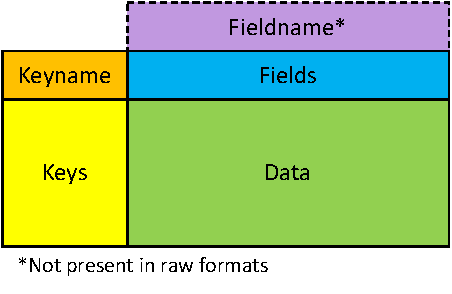
\includegraphics{table}
    \caption{The five properties of a table}
    \label{fig:table_props}
\end{figure}
\clearpage
\section{Creating Table Objects}
Table objects are created from the \cmdlink{tdatbl} class using the standard methods \textit{new} or \textit{create}. 
Once created, table objects act as commands with an ensemble of subcommands, or methods. 
These objects can be copied with the method \methodlink[0]{tdatbl}{copy} and deleted with the method \methodlink[0]{tdatbl}{destroy}.
\begin{syntax}
\command{tdatbl} new \$arg1 \$arg2 ...\\
tdatbl create \$objectName \$arg1 \$arg2 ...
\end{syntax}
\begin{args}
\$objectName & Explicit name for object. \\
\$arg1 \$arg2 ... & Arguments to pass to \methodlink[0]{tdatbl}{define} method.
\end{args}

\begin{example}{Creating a table object}
\begin{lstlisting}
set tableObj [table new]
\end{lstlisting}
\end{example}
\subsection{Copying Table Objects}
The method \methodlink[0]{tdatbl}{copy} copies all the data from a table object to a new object.
\begin{syntax}
\method{tdatbl}{copy} <\$objectName>
\end{syntax}
\begin{args}
\$objectName & Explicit name for object. By default, returns an auto-generated name.
\end{args}

\subsection{Removing Table Objects}
The standard method \methodlink[0]{tdatbl}{destroy} removes a table object from the interpreter. 
\begin{syntax}
\method{tdatbl}{destroy}
\end{syntax}
\clearpage
\section{Table Definition}
The method \methodlink[0]{tdatbl}{define} sets the property values of a table, filtering the data or adding keys and fields as necessary. For example, if the keys are defined to be a subset of the current fields, it will filter the data to only include the key subset. 
Also, if the data is defined, all existing data will be wiped, and any new keys or fields will be added.
\begin{syntax}
\method{tdatbl}{define} <\$properties> <\$option \$value ...>
\end{syntax}
\begin{args}
\$properties & Dictionary of properties. Mutually exclusive with option-value syntax. \\
\$option & Property to set: ``keyname'', ``fieldname'', ``keys'', ``fields'' or ``data''. \\
\$value & Value to set property to.
\end{args}
The remaining examples in this documentation will use the table as defined below:
\begin{example}{Example Table}
\begin{lstlisting}
set tableObj [table new]
$tableObj define data {
    1 {x 3.44 y 7.11 z 8.67} 
    2 {x 4.61 y 1.81 z 7.63}
    3 {x 8.25 y 7.56 z 3.84}
    4 {x 5.20 y 6.78 z 1.11}
    5 {x 3.26 y 9.92 z 4.56}
}
\end{lstlisting}
\end{example}
\clearpage
\section{Table Property Query}
The method \methodlink[0]{tdatbl}{properties} simply returns a dictionary of the table properties, as defined with \methodlink{tdatbl}{define}.
Additionally, calling the table object without any arguments will return the table properties.
\begin{syntax}
\method{tdatbl}{properties}
\end{syntax}
\begin{example}{Getting table properties (and trimming a table)}
\begin{lstlisting}
puts [$tableObj properties]; # Automatically generates keys and fields
$tableObj define keys {1 2} fields x; # Trims data
puts [$tableObj properties]
puts [$tableObj]
\end{lstlisting}
\tcblower
\begin{lstlisting}
keyname key fieldname field keys {1 2 3 4 5} fields {x y z} data {1 {x 3.44 y 7.11 z 8.67} 2 {x 4.61 y 1.81 z 7.63} 3 {x 8.25 y 7.56 z 3.84} 4 {x 5.20 y 6.78 z 1.11} 5 {x 3.26 y 9.92 z 4.56}}
keyname key fieldname field keys {1 2} fields x data {1 {x 3.44} 2 {x 4.61}}
keyname key fieldname field keys {1 2} fields x data {1 {x 3.44} 2 {x 4.61}}
\end{lstlisting}
\end{example}

\subsection{Get Keyname and Fieldname}
The keyname and fieldname properties of a table can be accessed directly with their respective methods. 
\begin{syntax}
\method{tdatbl}{keyname}
\end{syntax}
\begin{syntax}
\method{tdatbl}{fieldname} 
\end{syntax}
\subsection{Get Keys and Fields}
The table keys and fields are ordered lists of the row and column names of the table. They can be queried with the methods \methodlink[0]{tdatbl}{keys} and \methodlink[0]{tdatbl}{fields}, respectively. In addition to just returning the lists of keys and fields, a pattern can be specified in the same style as the Tcl  \textit{string match} command.
\begin{syntax}
\method{tdatbl}{keys} <\$pattern>
\end{syntax}
\begin{syntax}
\method{tdatbl}{fields} <\$pattern>
\end{syntax}
\begin{args}
\$pattern & String matching pattern. Default returns all
\end{args}
\clearpage
\subsection{Get Table Data (Dictionary Form)}
The method \methodlink[0]{tdatbl}{data} returns the table data in unsorted dictionary form, where blanks are represented by missing dictionary entries. 
\begin{syntax}
\method{tdatbl}{data} <\$key>
\end{syntax}
\begin{args}
\$key & Key to get row dictionary from (default returns all rows).
\end{args}

\begin{example}{Getting table data}
\begin{lstlisting}
puts [$tableObj data]
puts [$tableObj data 3]
\end{lstlisting}
\tcblower
\begin{lstlisting}
1 {x 3.44 y 7.11 z 8.67} 2 {x 4.61 y 1.81 z 7.63} 3 {x 8.25 y 7.56 z 3.84} 4 {x 5.20 y 6.78 z 1.11} 5 {x 3.26 y 9.92 z 4.56}
x 8.25 y 7.56 z 3.84
\end{lstlisting}
\end{example}
\subsection{Get Table Data (Matrix Form)}
The method \methodlink[0]{tdatbl}{values} returns a matrix (list of rows) that represents the data in the table, where the rows correspond to the keys and the columns correspond to the fields. Missing entries are represented by blanks in the matrix. 
\begin{syntax}
\method{tdatbl}{values}
\end{syntax}
\begin{example}{Getting table values}
\begin{lstlisting}
puts [$tableObj values]
\end{lstlisting}
\tcblower
\begin{lstlisting}
{3.44 7.11 8.67} {4.61 1.81 7.63} {8.25 7.56 3.84} {5.20 6.78 1.11} {3.26 9.92 4.56}
\end{lstlisting}
\end{example}
\clearpage
\subsection{Get Table Dimensions}
The dimensions of a table, as in the number of keys and fields, can be accessed with the method \methodlink[0]{tdatbl}{shape}. Note that rows and columns with missing data will be counted.
\begin{syntax}
\method{tdatbl}{shape} <\$dim>
\end{syntax}
\begin{args}
\$dim & Dimension to take size along (default will return the number of rows and columns as a list) \\
&\quad 0: Number of rows \\
&\quad 1: Number of columns 
\end{args}
Alternatively, the number of rows can be queried with \methodlink{tdatbl}{height} and the number of columns can be queried with \methodlink{tdatbl}{width}.
\begin{syntax}
\method{tdatbl}{height}
\end{syntax}
\begin{syntax}
\method{tdatbl}{width}
\end{syntax}

\begin{example}{Getting table dimensions}
\begin{lstlisting}
puts [$tableObj shape]
puts [$tableObj height]
puts [$tableObj width]
\end{lstlisting}
\tcblower
\begin{lstlisting}
5 3
5
3
\end{lstlisting}
\end{example}
\clearpage
\subsection{Check Existence of Table Keys/Fields}
The existence of a table key, field, or combination of key/field can be queried with the method \methodlink[0]{tdatbl}{exists}. 
\begin{syntax}
\method{tdatbl}{exists} key \$key \\
\$tableObj exists field \$field \\
\$tableObj exists value \$key \$field
\end{syntax}
\begin{args}
\$key & Key to check. \\
\$field & Field to check.
\end{args}
\subsection{Find Table Keys/Fields}
The row or column index of a table key or field can be queried with the method \methodlink[0]{tdatbl}{find}. \\
If the key or field does not exist, returns -1.

\begin{syntax}
\method{tdatbl}{find} key \$key \\
\$tableObj find field \$field
\end{syntax}
\begin{args}
\$key & Key to find. \\
\$field & Field to find.
\end{args}

\subsection{Get Table Key/Field}
The table key or field corresponding with a row or column index (\texttt{end-\textit{integer}} format supported) can be queried with the methods \methodlink[0]{tdatbl}{key} and \methodlink[0]{tdatbl}{field}. 
\begin{syntax}
\method{tdatbl}{key} \$rid
\end{syntax}
\begin{syntax}
\method{tdatbl}{field} \$cid
\end{syntax}
\begin{args}
\$rid & Row index. \\
\$cid & Column index.
\end{args}
\clearpage

\section{Table Entry and Access}
Data entry and access to a table object can be done with single values with the methods \methodlink[0]{tdatbl}{set} and \methodlink[0]{tdatbl}{get}, entire rows with \methodlink[0]{tdatbl}{rset} and \methodlink[0]{tdatbl}{rget}, entire columns with \methodlink[0]{tdatbl}{cset} and \methodlink[0]{tdatbl}{cget}, or in matrix fashion with \methodlink[0]{tdatbl}{mset} and  \methodlink[0]{tdatbl}{mget}. 
If entry keys/fields do not exist, they are added to the table. 
Additionally, since blank values represent missing data, setting a value to blank effectively unsets the table entry, but does not remove the key or field. 
\subsection{Single Value Entry and Access}
The methods \methodlink[0]{tdatbl}{set} and \methodlink[0]{tdatbl}{get} allow for easy entry and access of single values in the table. 
Note that multiple field-value pairings can be used in \methodlink{tdatbl}{set}. 
\begin{syntax}
\method{tdatbl}{set} \$key \$field \$value ...
\end{syntax}
\begin{syntax}
\method{tdatbl}{get} \$key \$field
\end{syntax}
\begin{args}
\$key & Key of row to set/get data in/from. \\
\$field & Field of column to set/get data in/from. \\
\$value & Value to set. 
\end{args}
\begin{example}{Setting multiple values}
\begin{lstlisting}
$tableObj set 1 x 2.00 y 5.00 foo bar
puts [$tableObj data 1]
\end{lstlisting}
\tcblower
\begin{lstlisting}
x 2.00 y 5.00 z 8.67 foo bar
\end{lstlisting}
\end{example}
\clearpage
\subsection{Row Entry and Access}
The methods \methodlink[0]{tdatbl}{rset} and \methodlink[0]{tdatbl}{rget} allow for easy row entry and access.
Entry list length must match table width or be scalar.
\begin{syntax}
\method{tdatbl}{rset} \$key \$row
\end{syntax}
\begin{syntax}
\method{tdatbl}{rget} \$key
\end{syntax}
\begin{args}
\$key & Key of row to set/get. \\
\$row & List of values (or scalar) to set. 
\end{args}
\subsection{Column Entry and Access}
The methods \methodlink[0]{tdatbl}{cset} and \methodlink[0]{tdatbl}{cget} allow for easy column entry and access.
Entry list length must match table height or be scalar.
\begin{syntax}
\method{tdatbl}{cset} \$field \$column
\end{syntax}
\begin{syntax}
\method{tdatbl}{cget} \$field
\end{syntax}
\begin{args}
\$field & Field of column to set/get. \\
\$column & List of values (or scalar) to set. 
\end{args}
\subsection{Matrix Entry and Access}
The methods \methodlink[0]{tdatbl}{mset} and \methodlink[0]{tdatbl}{mget} allow for easy matrix-style entry and access.
Entry matrix size must match table size or be scalar.
Note that \methodlink{tdatbl}{mget} with no arguments is identical to \methodlink{tdatbl}{values}.
\begin{syntax}
\method{tdatbl}{mset} <\$keys \$fields> \$matrix
\end{syntax}
\begin{syntax}
\method{tdatbl}{mget} <\$keys \$fields>
\end{syntax}
\begin{args}
\$keys & List of keys to set/get (default all keys). \\
\$fields & List of keys to set/get (default all keys). \\
\$matrix & Matrix of values (or scalar) to set.
\end{args}

\clearpage

\section{Iterating Over Table Data}
Table data can be looped through, row-wise, with the method \methodlink[0]{tdatbl}{with}. 
Variables representing the key values and fields will be assigned their corresponding values, with blanks representing missing data. 
The variable representing the key (table keyname) is static, but changes made to field variables are reflected in the table. 
Unsetting a field variable or setting its value to blank unsets the corresponding data in the table. 
\begin{syntax}
\method{tdatbl}{with} \$body
\end{syntax}
\begin{args}
\$body & Code to execute.
\end{args}
\begin{example}{Iterating over a table, accessing and modifying field values}
\begin{lstlisting}
set a 20.0
$tableObj add fields q
$tableObj with {
    puts [list $key $x]; # access key and field value
    set q [expr {$x*2 + $a}]; # modify field value
}
puts [$tableObj cget q]]
\end{lstlisting}
\tcblower
\begin{lstlisting}
1 3.44
2 4.61
3 8.25
4 5.20
5 3.26
26.88 29.22 36.5 30.4 26.52
\end{lstlisting}
\end{example}
Note: Just like in \textit{dict with}, the key variable and field variables in \methodlink{tdatbl}{with} persist after the loop.
\clearpage
\section{Field Expressions}
The method \methodlink[0]{tdatbl}{expr} computes a list of values according to a field expression. 
In the same style as referring to variables with the dollar sign (\$), the ``at'' symbol (@) is used by \methodlink{tdatbl}{expr} to refer to field values, or row keys if the keyname is used. 
If any referenced fields have missing values for a table row, the corresponding result will be blank as well. 
The resulting list corresponds to the keys in the table.
\begin{syntax}
\method{tdatbl}{expr} \$fieldExpr
\end{syntax}
\begin{args}
\$fieldExpr & Field expression.
\end{args}
\subsection{Editing Table Fields}
Field expressions can be used to edit existing fields or add new fields in a table with the method \methodlink[0]{tdatbl}{fedit}. 
If any of the referenced fields are blank, the corresponding entry will be blank as well.
\begin{syntax}
\method{tdatbl}{fedit} \$field \$fieldExpr
\end{syntax}
\begin{args}
\$field & Field to set. \\
\$fieldExpr & Field expression.
\end{args}
\begin{example}{Using field expressions}
\begin{lstlisting}
set a 20.0
puts [$tableObj cget x]
puts [$tableObj expr {@x*2 + $a}]
$tableObj fedit q {@x*2 + $a}
puts [$tableObj cget q]
\end{lstlisting}
\tcblower
\begin{lstlisting}
3.44 4.61 8.25 5.20 3.26
26.88 29.22 36.5 30.4 26.52
26.88 29.22 36.5 30.4 26.52
\end{lstlisting}
\end{example}
\clearpage
\subsection{Querying Keys that Match Criteria}
The method \methodlink[0]{tdatbl}{filter} returns the keys in a table that match criteria in a field expression.
\begin{syntax}
\method{tdatbl}{query} \$fieldExpr
\end{syntax}
\begin{args}
\$fieldExpr & Field expression that results in boolean value (true or false, 1 or 0).
\end{args}
\begin{example}{Getting keys that match criteria}
\begin{lstlisting}
puts [$tableObj query {@x > 3.0 && @y > 7.0}]
\end{lstlisting}
\tcblower
\begin{lstlisting}
1 3 5
\end{lstlisting}
\end{example}

\subsection{Filtering Table Based on Criteria}
The method \methodlink[0]{tdatbl}{filter} filters a table to the keys matching criteria in a field expression. 
\begin{syntax}
\method{tdatbl}{filter} \$fieldExpr
\end{syntax}
\begin{args}
\$fieldExpr & Field expression that results in boolean value (true or false, 1 or 0).
\end{args}
\begin{example}{Filtering table to only include keys that match criteria}
\begin{lstlisting}
$tableObj filter {@x > 3.0 && @y > 7.0}
puts [$tableObj keys]
\end{lstlisting}
\tcblower
\begin{lstlisting}
1 3 5
\end{lstlisting}
\end{example}

\clearpage

\section{Searching a Table}
Besides searching for specific field expression criteria with \methodlink{tdatbl}{query}, keys matching criteria can be found with the method \methodlink[0]{tdatbl}{search}. 
The method \methodlink[0]{tdatbl}{search} searches a table using the Tcl \textit{lsearch} command on the keys or field values. The default search method uses glob pattern matching, and returns matching keys.
This search behavior can be changed with the various options, which are taken directly from the Tcl \textit{lsearch} command. 
Therefore, while brief descriptions of the options are provided here, they are explained more in depth in the Tcl documentation, with the exception of the -inline option.
The -inline option filters a table based on the search criteria.
\begin{syntax}
\method{tdatbl}{search} <\$option1 \$option2 ...> <\$field> \$value
\end{syntax}
\begin{args}
\$option1 \$option2 ... & Searching options. Valid options: \\
\quad -exact & \quad Compare strings exactly \\
\quad -glob & \quad Use glob-style pattern matching (default) \\
\quad -regexp & \quad Use regular expression matching \\
\quad -sorted & \quad Assume elements are in sorted order \\
\quad -all & \quad Get all matches, rather than the first match \\
\quad -not & \quad Negate the match(es) \\
\quad -ascii & \quad Use string comparison (default) \\
\quad -dictionary & \quad Use dictionary-style comparison \\
\quad -integer & \quad Use integer comparison \\
\quad -real & \quad Use floating-point comparison \\
\quad -nocase & \quad Search in a case-insensitive manner \\
\quad -increasing & \quad Assume increasing order (default) \\
\quad -decreasing & \quad Assume decreasing order \\
\quad -bisect & \quad Perform inexact match \\
\quad -inline & \quad Filter table instead of returning keys. \\
\quad -{}- & \quad Signals end of options \\
\$field  & Field to search. If blank, searches keys. \\
\$value & Value or pattern to search for
\end{args}
Note: If a field contains missing values, they will only be included in the search if the search options allow (e.g. blanks are included for string matching, but not for numerical matching).
\clearpage
\section{Sorting a Table}
The method \methodlink[0]{tdatbl}{sort} sorts a table by keys or field values. 
The default sorting method is in increasing order, using string comparison. 
This sorting behavior can be changed with the various options, which are taken directly from the Tcl \textit{lsort} command. 
Therefore, while brief descriptions of the options are provided here, they are explained more in depth in the Tcl documentation.
Note: If a field contains missing values, the missing values will be last, regardless of sorting options. 
\begin{syntax}
\method{tdatbl}{sort} <\$option1 \$option2 ...> <\$field1 \$field2 ...>
\end{syntax}
\begin{args}
\$option1 \$option2 ... & Sorting options. Valid options: \\
\quad -ascii & \quad Use string comparison (default) \\
\quad -dictionary & \quad Use dictionary-style comparison \\
\quad -integer & \quad Use integer comparison \\
\quad -real & \quad Use floating comparison \\
\quad -increasing & \quad Sort the list in increasing order (default) \\
\quad -decreasing & \quad Sort the list in decreasing order \\
\quad -nocase & \quad Compare in a case-insensitive manner \\
\quad -{}- & \quad Signals end of options \\
\$field1 \$field2 ...  & Fields to sort by (in order of sorting). If blank, sorts by keys.
\end{args}
\begin{example}{Searching and sorting}
\begin{lstlisting}
puts [$tableObj search -real x 8.25]; # returns first matching key
$tableObj sort -real x
puts [$tableObj keys]
puts [$tableObj cget x]; # table access reflects sorted keys
puts [$tableObj search -sorted -bisect -real x 5.0]
\end{lstlisting}
\tcblower
\begin{lstlisting}
3
5 1 2 4 3
3.26 3.44 4.61 5.20 8.25
2
\end{lstlisting}
\end{example}
\clearpage
\section{Merging Tables}
Data from other tables can be merged into the table object with \methodlink{tdatbl}{merge}. 
In order to merge, all the tables must have the same keyname and fieldname. 
If the merge is valid, the table data is combined, with later entries taking precedence. 
Additionally, the keys and fields are combined, such that if a key appears in any of the tables, it is in the combined table.

\begin{syntax}
\method{tdatbl}{merge} \$arg1 \$arg2 ...
\end{syntax}
\begin{args}
\$arg1 \$arg2 ... & Other table objects to merge into table. Does not destroy the input tables. 
\end{args}

\begin{example}{Merging data from other tables}
\begin{lstlisting}
set newTable [table new]
$newTable set 1 x 5.00 q 6.34
$tableObj merge $newTable
$newTable destroy; # clean up
puts [$tableObj properties]
\end{lstlisting}
content...
\tcblower
\begin{lstlisting}
keyname key fieldname field keys {1 2 3 4 5} fields {x y z q} data {1 {x 5.00 y 7.11 z 8.67 q 6.34} 2 {x 4.61 y 1.81 z 7.63} 3 {x 8.25 y 7.56 z 3.84} 4 {x 5.20 y 6.78 z 1.11} 5 {x 3.26 y 9.92 z 4.56}}
\end{lstlisting}
\end{example}
\clearpage
\section{Table Manipulation}
The following methods are useful for adding, removing, and rearranging rows and columns in a table.
With the exception of \methodlink{tdatbl}{remove}, which removes corresponding data, and \methodlink{tdatbl}{mkkey}, which may cause data loss, these methods do not add or remove data, they only modify the key and field lists. 

\subsection{Adding Keys/Fields}
The method \methodlink[0]{tdatbl}{add} adds keys or fields to a table, appending to the end of the key/field lists. If a key or field already exists it is ignored.

\begin{syntax}
\method{tdatbl}{add} keys \$arg1 \$arg1 ... \\
\$tableObj add fields \$field1 \$field2 ...
\end{syntax}
\begin{args}
\$key1 \$key2 ... & Keys to add. \\
\$field1 \$field2 ... & Fields to add.
\end{args}

\subsection{Removing Keys/Fields}
The method  \methodlink[0]{tdatbl}{remove} removes keys or fields and their corresponding rows and columns from a table. If a key or field does not exist, it is ignored. 

\begin{syntax}
\method{tdatbl}{remove} keys \$key1 \$key2 ... \\
\$tableObj remove fields \$field1 \$field2 ...
\end{syntax}
\begin{args}
\$key1 \$key2 ... & Keys to remove. \\
\$field1 \$field2 ... & Fields to remove.
\end{args}

\subsection{Cleaning a Table}
Keys and fields with no data are removed with the method \methodlink[0]{tdatbl}{clean}. 
\begin{syntax}
\method{tdatbl}{clean}
\end{syntax}

\clearpage
\subsection{Inserting Keys/Fields}
The method  \methodlink[0]{tdatbl}{insert} inserts keys or fields at a specific row or column index. Input keys or fields must be unique and must not already exist. 

\begin{syntax}
\method{tdatbl}{insert} keys \$rid \$key1 \$key2 ... \\
\$tableObj insert fields \$cid \$field1 \$field2 ...
\end{syntax}
\begin{args}
\$rid & Row index to insert keys at. \\
\$key1 \$key2 ... & Keys to remove. \\
\$cid & Column index to insert fields at. \\
\$field1 \$field2 ... & Fields to remove.
\end{args}

\subsection{Renaming Keys/Fields}
The method  \methodlink[0]{tdatbl}{rename} renames keys or fields. Old keys and fields must exist. Duplicates are not allowed in old and new key/field lists.

\begin{syntax}
\method{tdatbl}{rename} keys \$oldKeys \$newKeys \\
\$tableObj rename fields \$oldFields \$newFields
\end{syntax}
\begin{args}
\$oldKeys & Keys to rename. Must exist. \\
\$newKeys & New key names. Must be same length as \$oldKeys. \\
\$oldFields & Fields to rename. Must exist. \\
\$newFields & New field names. Must be same length as \$oldFields.
\end{args}

\subsection{Making a Field the Key of a Table}
The method \methodlink[0]{tdatbl}{mkkey} makes a field the key of a table, and makes the key a field. 
If a field is empty for some keys, those keys will be lost. 
Additionally, if field values repeat, only the last entry for that field value will be included. 
This method is intended to be used with a field that is full and unique, and if the keyname matches a field name, this command will return an error.
\begin{syntax}
\method{tdatbl}{mkkey} \$field
\end{syntax}
\begin{args}
\$field & Field to swap with key.
\end{args}

\subsection{Swapping Rows/Columns}
Existing rows and columns can be swapped with the methods \methodlink[0]{tdatbl}{rswap} and \methodlink[0]{tdatbl}{cswap}.

\begin{syntax}
\method{tdatbl}{rswap} \$key1 \$key2
\end{syntax}
\begin{syntax}
\method{tdatbl}{cswap} \$field1 \$field2
\end{syntax}
\begin{args}
\$key1 \$key2 ... & Keys to swap. \\
\$field1 \$field2 ... & Fields to swap.
\end{args}

\subsection{Moving Rows/Columns}
Existing rows and columns can be moved with the methods \methodlink[0]{tdatbl}{rmove} and \methodlink[0]{tdatbl}{cmove}.

\begin{syntax}
\method{tdatbl}{rmove} \$key \$rid
\end{syntax}
\begin{syntax}
\method{tdatbl}{cmove} \$field \$cid
\end{syntax}
\begin{args}
\$key & Key of row to move. \\
\$rid & Row index to move to. \\
\$field & Field of row to move. \\
\$cid & Column index to move to. \\
\end{args}

\subsection{Transposing a Table}
The method \methodlink[0]{tdatbl}{transpose} transposes the table, making the keys the fields and the fields the keys.
\begin{syntax}
\method{tdatbl}{transpose}
\end{syntax}

\begin{example}{Transposing a table}
\begin{lstlisting}
$tableObj transpose
puts [$tableObj properties]
\end{lstlisting}
\tcblower
\begin{lstlisting}
keyname field fieldname key keys {x y z} fields {1 2 3 4 5} data {x {1 3.44 2 4.61 3 8.25 4 5.20 5 3.26} y {1 7.11 2 1.81 3 7.56 4 6.78 5 9.92} z {1 8.67 2 7.63 3 3.84 4 1.11 5 4.56}}
\end{lstlisting}
\end{example}

    \cleartooddpage[\thispagestyle{empty}]
\chapter{Datatype Conversion and File Utilities}\label{io}
\moduleinfo{io}
The ``io'' module provides datatype conversion, and file utilities for data import/export.
Four datatypes are supported by the ``io'' module: space-delimited values (txt), comma-separated values (csv), nested Tcl lists, or matrices (mat), and Tda tables (tbl). 
\clearpage

\section{Data Conversion}
The ``io'' module provides conversion utilities for different datatypes.  The intermediate format for Tda data conversion is matrix, or \textbf{mat}. 
\subsection{Matrix (mat)}
The matrix (\textbf{mat}) datatype is a nested Tcl list, where each list element represents a row vector of equal length. The ``io'' module is based around the \textbf{mat} datatype. An example of a matrix with headers is shown below. 
\begin{example}{Example Data (\textbf{mat}):}
\begin{lstlisting}
{step disp force} {1 0.02 4.5} {2 0.03 4.8} {3 0.07 12.6}
\end{lstlisting}
\end{example}
This format can be converted from and to all other formats, as is illustrated in the diagram below, with ``a'' \& ``b'' acting as placeholders for all other datatypes.
\begin{center}
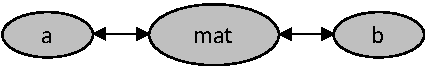
\includegraphics{dataconversion}
\end{center}
This way, each new datatype only requires the addition of two new conversion commands: one to \textbf{mat} and one from \textbf{mat}.
\clearpage
\subsection{Table (tbl)}
The table (\textbf{tbl}) datatype represents tabular data with row and column names, and are created and manipulated with the table module. 
If headers or row names are not used for  when converting to tabular data, default keys and fields will be generated, with keys starting at 1 and fields starting at ``A''.
To convert between ``mat'' \& ``tbl'', use the commands \cmdlink{mat2tbl} \& \cmdlink{tbl2mat}.
\begin{syntax}
\command{mat2tbl} \$matrix <\$hRow> <\$hCol>
\end{syntax}
\begin{args}
\$matrix & Matrix (row-oriented list of lists) \\
\$hRow & Whether to use first row of the matrix as fields. Default true \\
\$hCol & Whether to use the first column of the matrix as keys. Default true
\end{args}
\begin{syntax}
\command{tbl2mat} \$tblObj <\$hRow> <\$hCol>
\end{syntax}
\begin{args}
\$tblObj & Tda table object name \\
\$hRow & Whether to include fields as first row in matrix. Default true \\
\$hCol & Whether to include keys as first column in matrix. Default true
\end{args}
\clearpage
\subsection{Space-Delimited Text (txt)}
The space-delimited text (\textbf{txt}) datatype is simply space-delimited values, where new lines separate rows. 
Escaping of spaces and newlines is consistent with Tcl rules for valid lists. 
An example of the same data from the matrix example in \textbf{txt} format is shown below.
\begin{example}{Example Data (\textbf{txt}):}
\begin{lstlisting}
step disp force
1 0.02 4.5
2 0.03 4.8
3 0.07 12.6
\end{lstlisting}
\end{example}
To convert between \textbf{mat} \& \textbf{txt}, use the commands \cmdlink{mat2txt} \& \cmdlink{txt2mat}. 
\begin{syntax}
\command{mat2txt} \$matrix <\$hRow> <\$hCol>
\end{syntax}
\begin{args}
\$matrix & Matrix (row-oriented list of lists) \\
\$hRow & Whether to include header row. Default true \\
\$hCol & Whether to include header column. Default true
\end{args}
\begin{syntax}
\command{txt2mat} \$txt <\$hRow> <\$hCol>
\end{syntax}
\begin{args}
\$txt & Space \& newline-delimited table \\
\$hRow & Whether to include header row. Default true \\
\$hCol & Whether to include header column. Default true
\end{args}
\clearpage
\subsection{Comma-Separated Values (csv)}
The comma-separated values (\textbf{csv}) datatype is comma delimited values, where new lines separate rows. 
Commas and newlines are escaped with quotes, and quotes are escaped with double-quotes. 
An example of the same data from the matrix example in \textbf{csv} format is shown below.
\begin{example}{Example Data (\textbf{csv}):}
\begin{lstlisting}
step,disp,force
1,0.02,4.5
2 0.03,4.8
3,0.07,12.6
\end{lstlisting}
\end{example}
To convert between \textbf{mat} \& \textbf{csv}, use the commands \cmdlink{mat2csv} \& \cmdlink{csv2mat}. 
\begin{syntax}
\command{mat2csv} \$matrix <\$hRow> <\$hCol>
\end{syntax}
\begin{args}
\$matrix & Matrix \\
\$hRow & Whether to include header row. Default true \\
\$hCol & Whether to include header column. Default true
\end{args}
\begin{syntax}
\command{csv2mat} \$csv <\$hRow> <\$hCol>
\end{syntax}
\begin{args}
\$csv & Comma-separated values (with escaped commas, newlines, and quotes) \\
\$hRow & Whether to include header row. Default true \\
\$hCol & Whether to include header column. Default true
\end{args}
\clearpage
\subsection{Conversion Shortcuts}
Using the \textbf{mat} datatype as the intermediate datatype, data can be converted to and from any datatype, as is shown in the example below. 
\begin{example}{Example Code (using \textbf{mat} as intermediate):}
\begin{lstlisting}
set txt {step disp force
1 0.02 4.5
2 0.03 4.8
3 0.07 12.6}
set matrix [txt2mat $txt]
set csv [mat2csv $matrix]
puts $csv
\end{lstlisting}
\tcblower
\begin{lstlisting}
step,disp,force
1,0.02,4.5
2,0.03,4.8
3,0.07,12.6
\end{lstlisting}
\end{example}
For data conversions that use matrix as an intermediate format, shortcut commands are provided, illustrated in the table below. The optional arguments \texttt{\$hRow} \& \texttt{\$hCol} are the same for the shortcut conversion commands.
\begin{center}
\begin{tabular}{|r|c|c|c|}
\hline
& \textbf{txt} & \textbf{csv} & \textbf{tbl} \\
\hline
\textbf{txt} & \cellcolor{gray} & \command{txt2csv} & \command{txt2tbl} \\
\hline
\textbf{csv} & \command{csv2txt} &  \cellcolor{gray} & \command{csv2tbl} \\
\hline
\textbf{tbl} & \command{tbl2txt} & \command{tbl2csv} & \cellcolor{gray} \\
\hline
\end{tabular}
\end{center}
\clearpage
\section{File Utilities}
The commands \cmdlink{readFile}, \cmdlink{writeFile}, and \cmdlink{appendFile} simplify reading and writing of files in Tcl. Syntax is inspired from similar commands in the Tcllib fileutil package.
\begin{syntax}
\command{readFile} <\$option \$value ...> <-newline> \$filename
\end{syntax}
\begin{args}
\$option \$value ... & File configuration options, see Tcl \textit{fconfigure} command. \\
-nonewline & Option to read the final newline if it exists. \\
\$filename & File to read data from.
\end{args}
\begin{syntax}
\command{writeFile} <\$option \$value ...> <-nonewline> \$filename \$data
\end{syntax}
\begin{args}
\$option \$value ... & File configuration options, see Tcl \textit{fconfigure} command. \\
-nonewline & Option to not write a final newline. \\
\$filename & File to write data to. \\
\$data & Data to write to file.
\end{args}
\begin{syntax}
\command{appendFile} <\$option \$value ...> <-nonewline> \$filename \$data
\end{syntax}
\begin{args}
\$option \$value ... & File configuration options, see Tcl \textit{fconfigure} command. \\
-nonewline & Option to not write a final newline. \\
\$filename & File to append data to. \\
\$data & Data to append to file.
\end{args}
\begin{example}[label=ex:import_export]{File import/export}
\begin{lstlisting}
# Export data to file (creates or overwrites the file)
writeFile example.txt "hello world"
appendFile example.txt "goodbye moon"
# Import the contents of the file (requires that the file exists)
puts [readFile example.txt]
\end{lstlisting}
\tcblower
\begin{lstlisting}
hello world
goodbye moon
\end{lstlisting}
\end{example}
\clearpage
\section{Data Import and Export Shortcuts}
In addition to the fundamental file utilities and data conversion commands, the ``data'' module also provides some shortcut commands for common data import and export workflows.
\subsection{Matrix Import and Export}
The commands \cmdlink{readMatrix} and \cmdlink{writeMatrix} read/write a matrix from/to a file, converting from/to \textbf{csv} if the extension is .csv, and converting from/to \textbf{txt} otherwise.
Except for the input argument \texttt{\$matrix}, the input arguments are identical to \cmdlink{readFile} and \cmdlink{writeFile}.
\begin{syntax}
\command{readMatrix} <\$option \$value ...> <-newline> \$filename
\end{syntax}
\begin{syntax}
\command{writeMatrix} <\$option \$value ...> <-nonewline> \$filename \$matrix
\end{syntax}
\begin{args}
\$matrix & Matrix to convert and write to file.
\end{args}
\subsection{Table Import and Export}
The commands \cmdlink{readTable} and \cmdlink{writeTable} read/write a table from/to a file, converting from/to \textbf{csv} if the extension is .csv, and converting from/to \textbf{txt} otherwise.
Except for the input argument \texttt{\$table}, the input arguments are identical to \cmdlink{readFile} and \cmdlink{writeFile}.
\begin{syntax}
\command{readTable} <\$option \$value ...> <-newline> \$filename
\end{syntax}
\begin{syntax}
\command{writeTable} <\$option \$value ...> <-nonewline> \$filename \$table
\end{syntax}
\begin{args}
\$table & Table to convert and write to file.
\end{args}
\clearpage






    \cleartooddpage[\thispagestyle{empty}]
\chapter{Data Visualization}\label{vis}
\moduleinfo{vis}
The ``vis'' module provides utilities for viewing data in Tcl. It utilizes the ``wob'' package for managing Tk widgets, so in order to interact with the widgets, one must enter the Tcl/Tk event loop. The \textit{mainLoop} command in the ``wob'' package is an easy way to accomplish this.

\clearpage
\section{View tabular and matrix data}
Tda tables and matrices can be interactively explored with the commands \cmdlink{viewTable} and \cmdlink{viewMatrix}.

\begin{syntax}
viewTable \$tblObj
\end{syntax}
\begin{syntax}
viewMatrix \$matrix
\end{syntax}
\begin{args}
\$tblObj & Object name of Tda table object. \\
\$matrix  & Matrix to view. 
\end{args}
\begin{example}{Viewing tabular and matrix data}
\begin{lstlisting}
set tblObj [tbl new]
$tblObj define data {
    1 {x 3.44 y 7.11 z 8.67}
    2 {x 4.61 y 1.81 z 7.63}
    3 {x 8.25 y 7.56 z 3.84}
    4 {x 5.20 y 6.78 z 1.11}
    5 {x 3.26 y 9.92 z 4.56}
}
viewTable $tblObj
viewMatrix [$tblObj values]
wob::mainLoop
\end{lstlisting}
\end{example}
\begin{figure}[!htb]
\centering
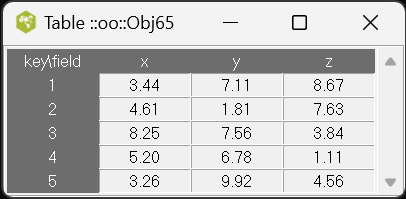
\includegraphics[width=0.4\linewidth]{viewtable}
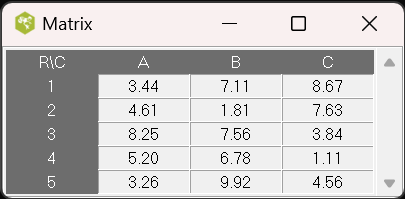
\includegraphics[width=0.4\linewidth]{viewmatrix}
\caption{Interactive table and matrix viewer}
\label{fig:viewdata}
\end{figure}

\clearpage
\section{Plot XY data}
XY data can be explored graphically with the command \cmdlink{plotXY}. Use the arrow keys or slider to move through the data, and use the scroll wheel on the mouse to switch between data series.
This widget was inspired from ``plotpoints'' on the Tcl wiki: \url{https://wiki.tcl-lang.org/page/A+little+function+plotter}.
\begin{syntax}
\cmdlink{figure} \$XY \\
figure \$X \$Y1 \$Y2 ...
\end{syntax}
\begin{args}
\$XY & Two-column matrix, first column X, second column Y1, third column Y2, etc. \\
\$X \$Y1 \$Y2 ... & X and Y vectors of the same length, mutually exclusive with \texttt{\$XY}. 
\end{args}
\begin{example}{Creating a figure object}
\begin{lstlisting}
namespace path ::tcl::mathfunc
set x [linsteps 0.01 -10 10]
set y [vmap sin $x]
plotXY $x $y
wob::mainLoop
\end{lstlisting}
\end{example}
\begin{figure}[!htb]
\centering
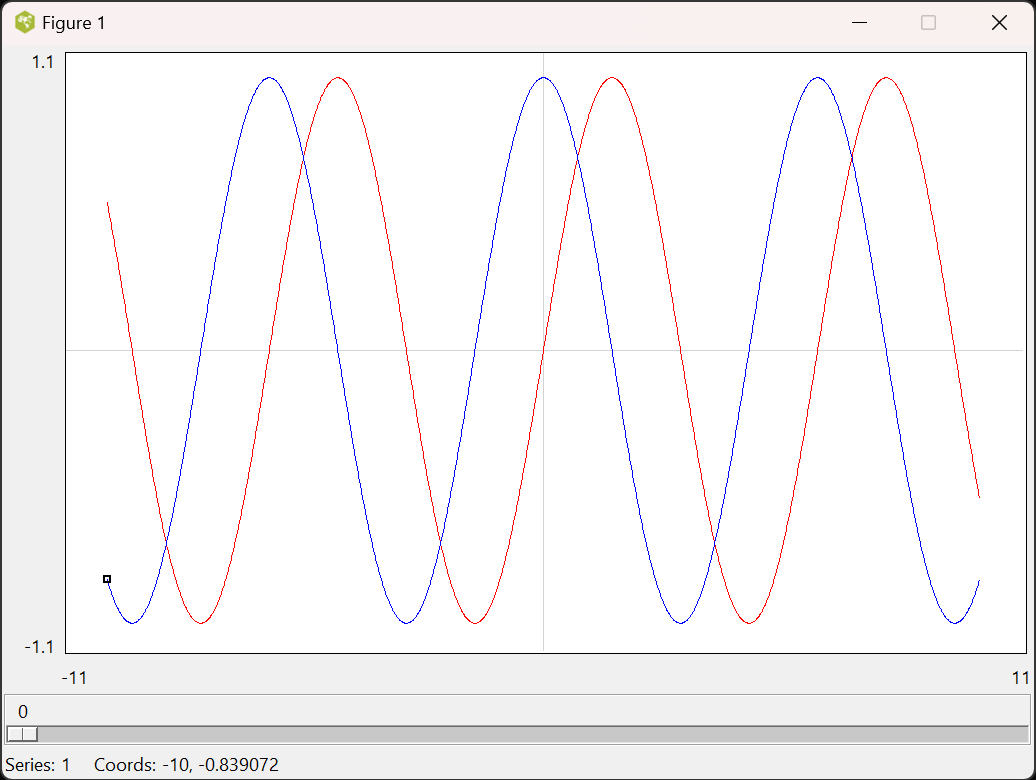
\includegraphics[width=0.7\linewidth]{plot}
\caption{Example XY plot}
\label{fig:plot}
\end{figure}

    \phantomsection
\interlinepenalty=1000
\printbibliography[heading=bibintoc]
    \cleartooddpage[\thispagestyle{empty}]
    \phantomsection
    \titleformat{\chapter}{\sffamily\bfseries\Huge}{}{0pt}{}
    \printindex
\end{document}